\documentclass[]{book}

%These tell TeX which packages to use.
\usepackage{array,epsfig}
\usepackage{amsmath}
\usepackage{amsfonts}
\usepackage{amssymb}
\usepackage{amsxtra}
\usepackage{amsthm}
\usepackage{mathrsfs}
\usepackage{color}

%Here I define some theorem styles and shortcut commands for symbols I use often
\theoremstyle{definition}
\newtheorem{defn}{Definition}
\newtheorem{thm}{Theorem}
\newtheorem{cor}{Corollary}
\newtheorem*{rmk}{Remark}
\newtheorem{lem}{Lemma}
\newtheorem*{joke}{Joke}
\newtheorem{ex}{Example}
\newtheorem*{soln}{Solution}
\newtheorem{prop}{Proposition}

\newcommand{\lra}{\longrightarrow}
\newcommand{\ra}{\rightarrow}
\newcommand{\surj}{\twoheadrightarrow}
\newcommand{\graph}{\mathrm{graph}}
\newcommand{\bb}[1]{\mathbb{#1}}
\newcommand{\Z}{\bb{Z}}
\newcommand{\Q}{\bb{Q}}
\newcommand{\R}{\bb{R}}
\newcommand{\C}{\bb{C}}
\newcommand{\N}{\bb{N}}
\newcommand{\M}{\mathbf{M}}
\newcommand{\m}{\mathbf{m}}
\newcommand{\MM}{\mathscr{M}}
\newcommand{\HH}{\mathscr{H}}
\newcommand{\Om}{\Omega}
\newcommand{\Ho}{\in\HH(\Om)}
\newcommand{\bd}{\partial}
\newcommand{\del}{\partial}
\newcommand{\bardel}{\overline\partial}
\newcommand{\textdf}[1]{\textbf{\textsf{#1}}\index{#1}}
\newcommand{\img}{\mathrm{img}}
\newcommand{\ip}[2]{\left\langle{#1},{#2}\right\rangle}
\newcommand{\inter}[1]{\mathrm{int}{#1}}
\newcommand{\exter}[1]{\mathrm{ext}{#1}}
\newcommand{\cl}[1]{\mathrm{cl}{#1}}
\newcommand{\ds}{\displaystyle}
\newcommand{\vol}{\mathrm{vol}}
\newcommand{\cnt}{\mathrm{ct}}
\newcommand{\osc}{\mathrm{osc}}
\newcommand{\LL}{\mathbf{L}}
\newcommand{\UU}{\mathbf{U}}
\newcommand{\support}{\mathrm{support}}
\newcommand{\AND}{\;\wedge\;}
\newcommand{\OR}{\;\vee\;}
\newcommand{\Oset}{\varnothing}
\newcommand{\st}{\ni}
\newcommand{\wh}{\widehat}

%Pagination stuff.
\setlength{\topmargin}{-.3 in}
\setlength{\oddsidemargin}{0in}
\setlength{\evensidemargin}{0in}
\setlength{\textheight}{9.in}
\setlength{\textwidth}{6.5in}
\pagestyle{empty}



\begin{document}


\begin{center}
{\Large{ \textbf{Reviews of Stochastic Gradient Descent Variants and its Asychonous Version}}}\\
\end{center}

\vspace{0.2 cm}


% \subsection*{Exercises for Section 1.1: Norm and Inner Product} star means no numbers
\subsection*{Introduction}
In this review, we will introduce several at start-of-art gradient descent optimization algorthims.In full gradient descent optimization, we compute the cost gradient based on the complete training set. In case of very large datasets, using full gradient descent can be quite costly since we are only taking a single step for one pass overIn full gradient descent optimization, we compute the cost gradient based on the complete training set. In case of very large datasets, using full gradient descent can be quite costly since we are only taking a single step for one pass over
\subsection*{Notation}
At first we introduce some notations about convex optimization.\\
\textbf{Convex Function}\\
A function $f : \mathbb{R}^n \to \mathbb{R}$ is convex, if: $$f(\alpha x + (1-\alpha)y) \le \alpha f(x)+(1-\alpha)f(y),\forall x,y \in \mathbb{R}^n, \forall \alpha \in (0,1)$$
\begin{figure}[h]
\begin{center}
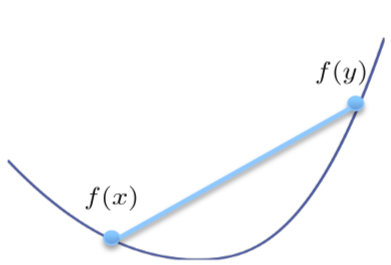
\includegraphics[width=0.3\textwidth]{convex} % Include the image placeholder.png

\end{center}
\end{figure}\\
And it also means (Suppose $f$ is differentiable) $$f(y)\ge f(x)+\nabla f(x)^T(y-x),\forall x,y\in\mathbb{R}^n$$
\begin{figure}[h]
\begin{center}
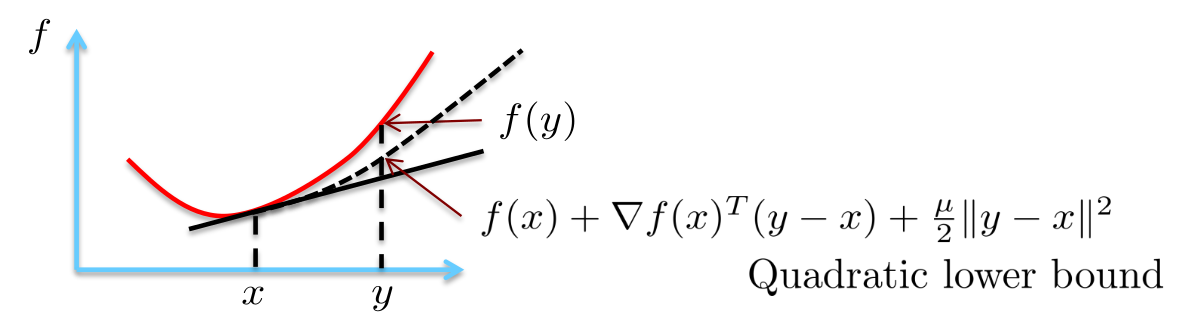
\includegraphics[width=0.6\textwidth]{convex1} % Include the image placeholder.png

\end{center}
\end{figure}\\
\textbf{Strong Convexity}\\
A differentiable function $f$ is strongly convex if\\
$$f(y)\ge f(x)+\nabla f(x)^T(y-x)+\frac{\mu}{2}\rVert y-x \rVert^2,\forall x,y\in\mathbb{R}^n$$\\
\begin{figure}[!htbp]
\begin{center}
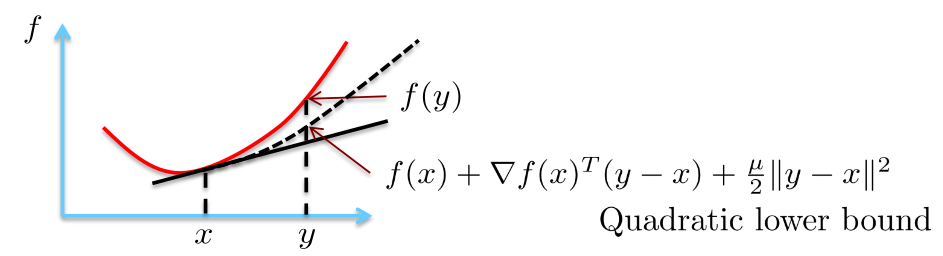
\includegraphics[width=0.6\textwidth]{strong} % Include the image placeholder.png

\end{center}
\end{figure}\\
\textbf{Convex Function with Lipschitz Continuous}\\
Let $\nabla f$ be Lipschitz continuous, ie., there exitst $L \ge 0$ such that $$\rVert  \nabla f(x)- \nabla f(y)\rVert \le L \rVert x-y \rVert, \forall x,y \in \mathbb{R}^n $$
\begin{figure}[!htbp]
\begin{center}
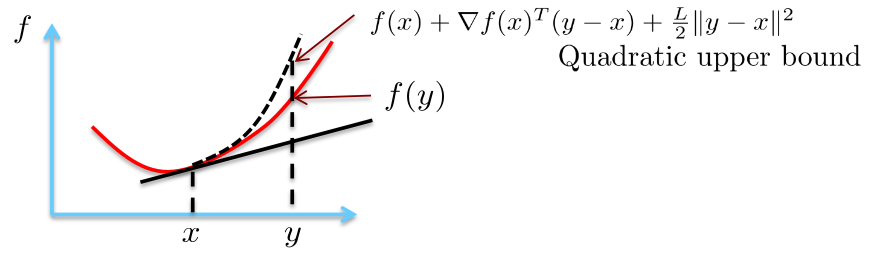
\includegraphics[width=0.6\textwidth]{convexL}
\end{center}
\end{figure}
\subsection*{Gradient Descent}
\textbf{Update Rule}\\
\textbf{Convergence Rate}\\
\subsection*{Stoastic Gradient Descent}
\subsection*{Stoastic Average Gradient Descent(SAG)}
\subsection*{Stoastic Gradient Descent with Predictive Variance Reduction(SVRG)}




\end{document}
